\begin{figure}[h]
  \hypertarget{RelatePFGICFHWCRICPFFVAC}{}
  \centerline{
    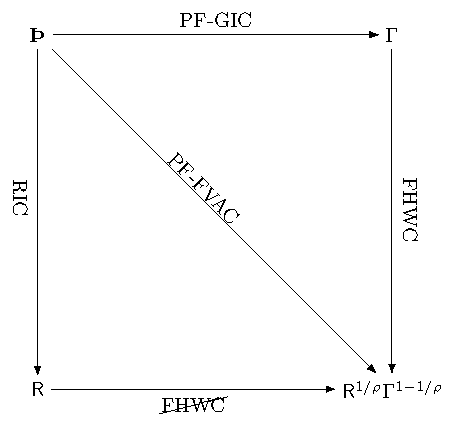
\includegraphics{\FigDir/RelatePFGICFHWCRICPFFVAC}
  }
  \caption{Relation of \PFGIC, \FHWC, \RIC, and \PFFVAC} \label{fig:RelatePFGICFHWCRICPFFVAC}
  \footnotesize{Arrows reflect the direction of the relationship; an arrowhead points to the larger of the two quantities being compared.  For example, the topmost arrow, pointing from $\Pat$ to $\PGro$ indicates that $\PGro > \Pat$.}
\end{figure}
